\subsection{Simulated rat hippocampal spike data in a navigation task}
\label{subsection:synthetic_results}

Using signed Ornstein--Uhlenbeck movement motivated by \citet{theodoni_2018_theta_ou}, we simulate a rat's position and velocity over 600 seconds on a linear 1-m track (\autoref{figure:task_overview}a), together with spike counts from $N=100$ neurons: four place cells~\citep{okeefe_dostrovsky_1971_place_cells} with varying peak firing rates and spatial extents, and 96 position-independent ``noise'' neurons (\autoref{figure:synthetic_results}a,b; \hyperref[subsubsection:synthetic_results_details]{\ref*{subsubsection:synthetic_results_details}} for details). The first two place fields are asymmetric and centered at 0.2 and 0.4 m; the other two are symmetric and centered at 0.7 m with differing widths (\autoref{figure:synthetic_rate_design}). The simulated neural data are processed into 50-ms binned spike counts per neuron.

We first verify that vanilla SED latents can recover known place cell activity from place cells 1 and 2 despite the presence of the noise neurons. Indeed, across five independently trained models (each with $S=1$, $D=128$, $B=1024$, $k=4$), we find latents with activations nearly identical to the place cells (\autoref{figure:synthetic_results}c).

We then ask whether a Matryoshka SED can additionally recover the activity associated with both the encompassing and nested place cells 3 and 4. Again, across five independently trained models (each with $S=1$, $(D_1,k_1)=(64,4)$, $(D_2,k_2)=(128,4)$, and $B=1024$), we find latents that recover both fields, with the broader and narrower place fields recovered in latents in the first and second Matryoshka levels respectively, as expected (\autoref{figure:synthetic_results}d).

Last, we evaluate whether a W-SED can find features that evolve over time in this setting, e.g., a feature that represents continuous movement. We train five FW-SEDs and five TW-SEDs over 1-s windows (each with $S=20$, $D=128$, $k=4$, $B=256$) and find latents that are active during 1 s of movement in particular directions. In \autoref{figure:synthetic_results}e we show for one particular TW-SED latent the position over time for activating examples, which clearly illustrates forward motion through place fields 1 and 2. We find that both FW-SEDs and TW-SEDs can find such features (\autoref{figure:synthetic_temporal_comparison}), with directional features recovered in more TW-SED runs. TW-SED latents exhibit preferences for both forward and backward movement (\autoref{figure:synthetic_temporal_features} and \autoref{figure:synthetic_ramp_conditioned}). We also examine the neural activity associated with spatial and temporal latents, finding positive attribution concentrated in the expected place cells and near-zero attribution for noise neurons (\autoref{figure:synthetic_unit_traceback} and \autoref{figure:synthetic_temporal_coactivity}), and quantify their selectivity for the expected spatial locations and movement directions (\hyperref[subsubsection:synthetic_results_details]{\ref*{subsubsection:synthetic_results_details}}). 

As a baseline comparison, we apply PCA to an $11{,}981\times2{,}000$ matrix of overlapping 1-s neural activity windows, with each row concatenating twenty 50-ms bins from all 100 neurons. We retain 128 principal components to match $D$ from the SED models above. We find that individual principal components exhibit mixed spatial tuning and do not cleanly separate any of the four place fields (\autoref{figure:synthetic_pca_spatial}). Interestingly, a single component can strongly distinguish forward from backward crossings through the first two fields, although its most extreme scores across the full recording are not selective for these traversals (\autoref{figure:synthetic_pca_direction}). Overall, these results demonstrate that NLDisco can cleanly recover known ground-truth features that a PCA baseline misses, and highlight the utility of each SED model that NLDisco provides.

\begin{figure}[tb]
    \centering
    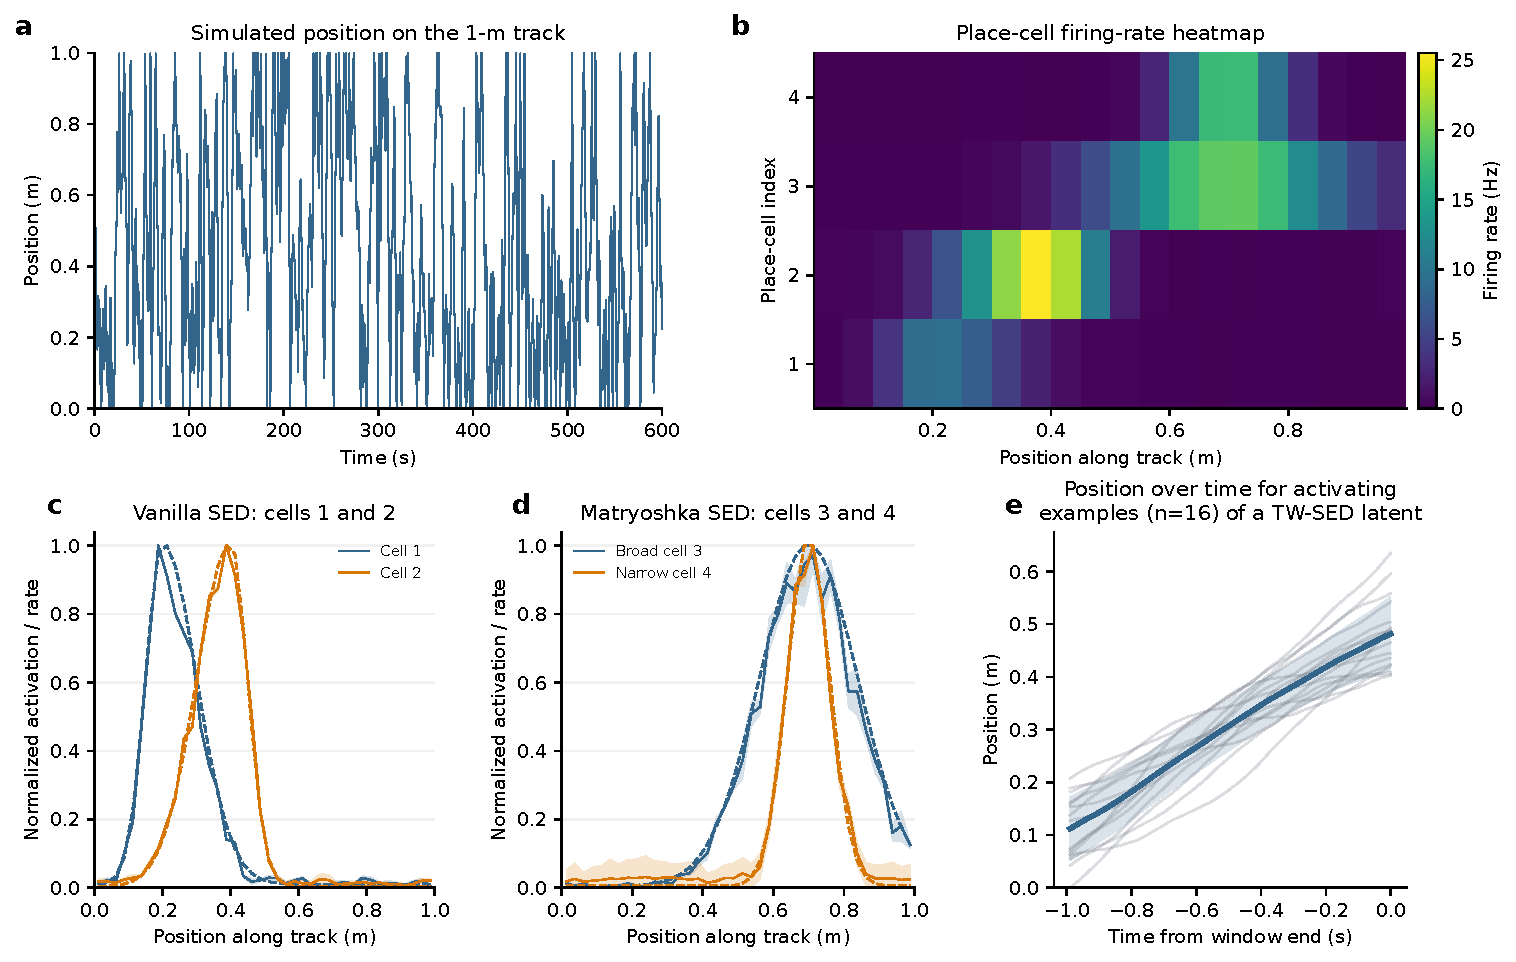
\includegraphics[width=\linewidth]{figures/figure3.pdf}
    \caption{
        \textbf{Spatial and temporal features recovered from a controlled simulation.} \\
        \small
        \textbf{(a)} Simulated position. \textbf{(b)} Empirical firing rates of the four simulated place cells in 20 spatial bins. \textbf{(c)} For each of five independent training runs with $S=1$, $D=128$, $k=4$, $B=1024$, SED latents identify the activity of place cells 1 and 2: solid curves and shaded bounds show the mean activation and $\pm1$ sample S.D. of the best matching latents; dashed curves show the exact place field. \textbf{(d)} For each of five independent Matryoshka SED fits with $S=1$, $(D_1,k_1)=(64,4)$, $(D_2,k_2)=(128,4)$, and $B=1024$, latents identify both broad and narrow place cells 3 and 4. Solid and dashed curves and shaded bounds same as in c. \textbf{(e)} Activating examples for an $S=20$, $D=128$, $k=4$, $B=256$ TW-SED latent that captures forward motion through place fields 1 and 2. Thin gray curves are individual trajectories, with mean (bold curve) and $\pm1$ sample S.D. (shaded bounds).
        \vspace{-1em}
    }
    \label{figure:synthetic_results}
\end{figure}
